% Exact mixed-qubit illustration; derivation in Appendix J.
\documentclass[tikz,border=2pt]{standalone}
\usepackage{fix-cm}
\usepackage[T1]{fontenc}
\usepackage{mathpazo}
\usepackage[default]{sourcesanspro}
\usepackage{pgfplots}
\usetikzlibrary{arrows.meta}
\pgfplotsset{compat=1.18}
\definecolor{Ink}{HTML}{25333A}
\definecolor{Muted}{HTML}{59656A}
\definecolor{Rule}{HTML}{D5DAD8}
\definecolor{Green}{HTML}{66C2A5}
\definecolor{Blue}{HTML}{8DA0CB}
\definecolor{GreenText}{HTML}{28634F}
\definecolor{BlueText}{HTML}{465A81}
\begin{document}
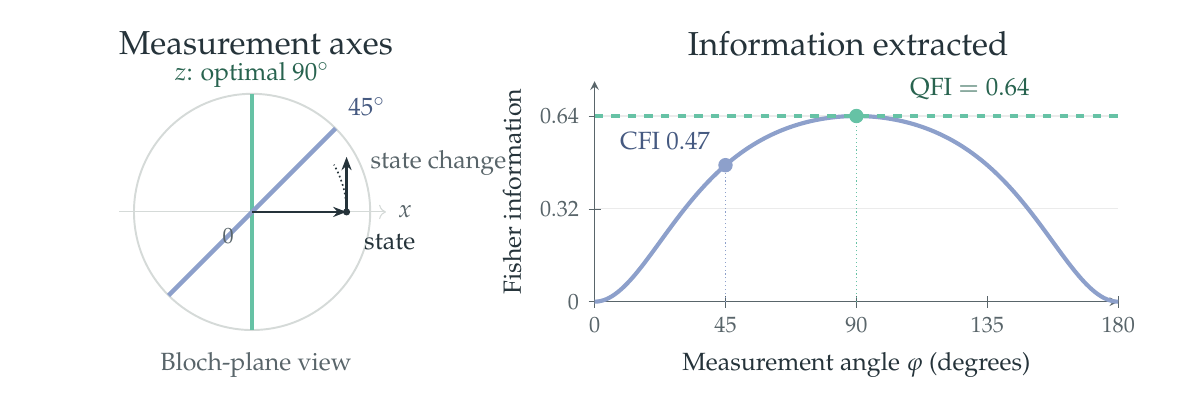
\begin{tikzpicture}[x=1cm,y=1cm]
 \path[use as bounding box] (0,0) rectangle (14.3,4.5);
 \node[font=\rmfamily\large,text=Ink] at (2.9,4.3) {Measurement axes};
 \node[font=\rmfamily\large,text=Ink] at (10.42,4.3) {Information extracted};
 \coordinate (o) at (2.85,2.16);
 \draw[Rule,line width=.7pt] (o) circle (1.5);
 \draw[Rule,->] (1.16,2.16)--(4.55,2.16);
 \node[font=\small,text=Muted,anchor=west] at (4.58,2.16) {$x$};
 \draw[Green,line width=1.6pt] (2.85,.66)--(2.85,3.66);
 \node[font=\small,text=GreenText,anchor=south] at (2.85,3.61) {$z$: optimal $90^\circ$};
 \draw[Blue,line width=1.6pt] (1.78934,1.09934)--(3.91066,3.22066);
 \node[font=\small,text=BlueText,anchor=south west] at (3.95,3.25) {$45^\circ$};
 \draw[Ink,-{Stealth[length=1.7mm]},line width=.9pt] (o)--(4.05,2.16);
 \fill[Ink] (4.05,2.16) circle (.045);
 \node[font=\small,text=Ink,anchor=north west] at (4.15,2.0) {state};
 \node[font=\footnotesize,text=Muted,anchor=north east] at (2.74,2.08) {$0$};
 \draw[Ink,densely dotted,line width=.6pt] (4.05,2.16) arc[start angle=0,end angle=30,radius=1.2];
 \draw[Ink,-{Stealth[length=1.7mm]},line width=.8pt] (4.05,2.16)--(4.05,2.86);
 \node[font=\small,text=Muted,anchor=west,align=left] at (4.23,2.78) {state change};
 \node[font=\small,text=Muted,align=center] at (2.9,.22) {Bloch-plane view};
 \begin{axis}[at={(7.2cm,1.02cm)},anchor=south west,width=6.65cm,height=2.8cm,scale only axis,
  xmin=0,xmax=180,ymin=0,ymax=.76,
  axis lines=left,axis line style={Muted},tick style={Muted},
  xtick={0,45,90,135,180},ytick={0,.32,.64},yticklabels={$0$,$0.32$,$0.64$},
  tick label style={font=\footnotesize,text=Muted},
  xlabel={Measurement angle $\varphi$ (degrees)},ylabel={Fisher information},
  xlabel style={font=\small,text=Ink},ylabel style={font=\small,text=Ink},
  ymajorgrids=true,grid style={black!8},clip=false]
  \addplot[Blue,line width=1.5pt,domain=0:180,samples=181] {.64*sin(x)^2/(1-.64*cos(x)^2)};
  \addplot[Green,dashed,line width=1.4pt,domain=0:180] {.64};
  \draw[Blue,densely dotted] (axis cs:45,0)--(axis cs:45,.4705882353);
  \draw[Green,densely dotted] (axis cs:90,0)--(axis cs:90,.64);
  \addplot[only marks,mark=*,mark size=2.4pt,Blue] coordinates {(45,.4705882353)};
  \addplot[only marks,mark=*,mark size=2.4pt,Green] coordinates {(90,.64)};
  \node[font=\small,text=BlueText,anchor=south east] at (axis cs:43,.49) {CFI $0.47$};
  \node[font=\small,text=GreenText,anchor=south] at (axis cs:129,.66) {QFI $=0.64$};
 \end{axis}
\end{tikzpicture}
\end{document}
